\chapter{Il percorso di stage }\label{cap:Il_percorso}
\section{Formazione}
Il processo di formazione che mi è stato fornito ha avuto un ruolo fondamentale nella buona riuscita del progetto di stage, 
ha avuto una durata di circa 4 settimane. \\
La causa del protrarsi del processo di formazione è stata provocata dal fatto che concetti legati all'architettura \gls{eda}{},
\textbf{Apache Kafka}, \textbf{Apache Druid}, \textbf{Docker Compose} sono state del tutto innovative per me.\\
Tutto il processo di formazione è stato tracciato e monitorato dal tutor aziendale e da me stesso attraverso le \gls{board}{} offerte 
dal software di project management \textbf{ClickUp} (Figura \ref{cap:ClickUp}).\\
\begin{figure}[h]
    \centering
    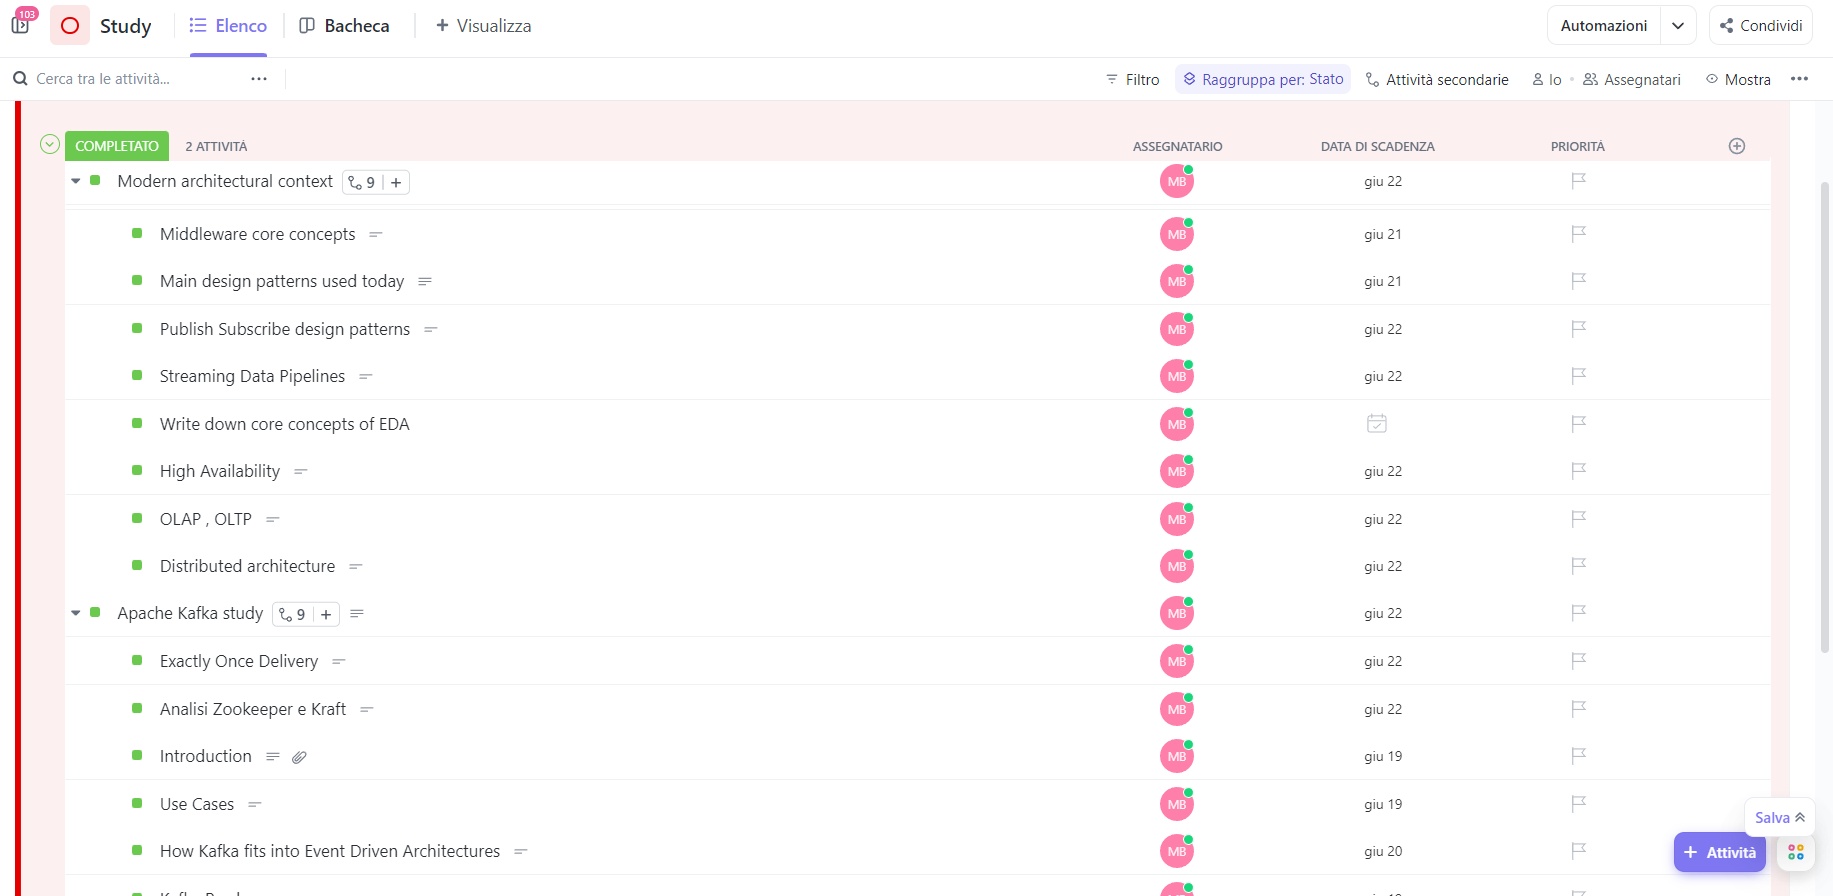
\includegraphics[width=1\textwidth]{images/percorso/formazione.png}
    \caption{Board di ClickUp per il processo di formazione}
    \label{cap:ClickUp}
\end{figure}
\pagebreak
\\
Inoltre durante il processo di formazione, oltre a reperire informazioni da documentazione ufficiale fornita , ho avuto anche modo 
di approfondire quanto appena appreso attraverso delle attività di \gls{hands-on}{} che mi hanno permesso di mettere in pratica quanto appreso (Figura \ref{cap:Hands-on}).
\begin{figure}[h]
    \centering
    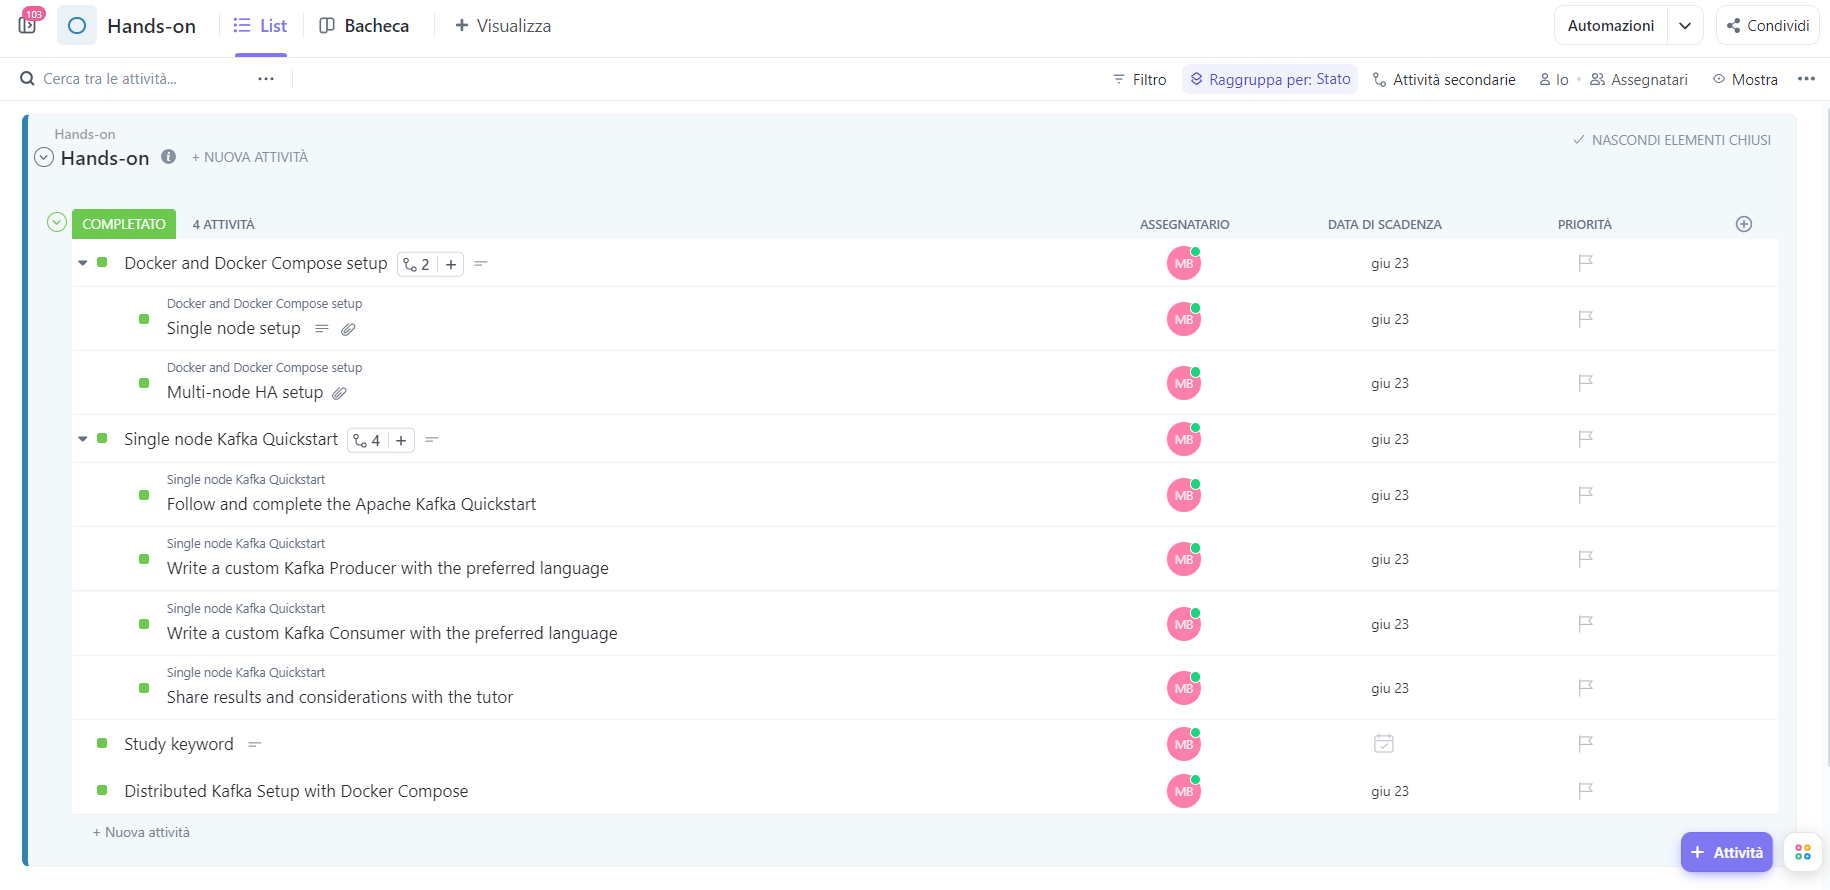
\includegraphics[width=1\textwidth]{images/percorso/hands_on.png}
    \caption{Attività di hands-on per il processo di formazione}
    \label{cap:Hands-on}
\end{figure}
\\
Oltre a ciò, durante il processo di formazione, in collaborazione con il tutor aziendale, è stato definito un processo di coordinamento e produzione di 
documentazione tecnica che mi ha permesso durante tutto lo svolgimento del percorso di stage di avere un tracciamento dei concetti appresi 
e di avere riferimenti per la risoluzione di problemi o dubbi sorti (Figura \ref{cap:Documentazione})
\begin{figure}[h]
    \centering
    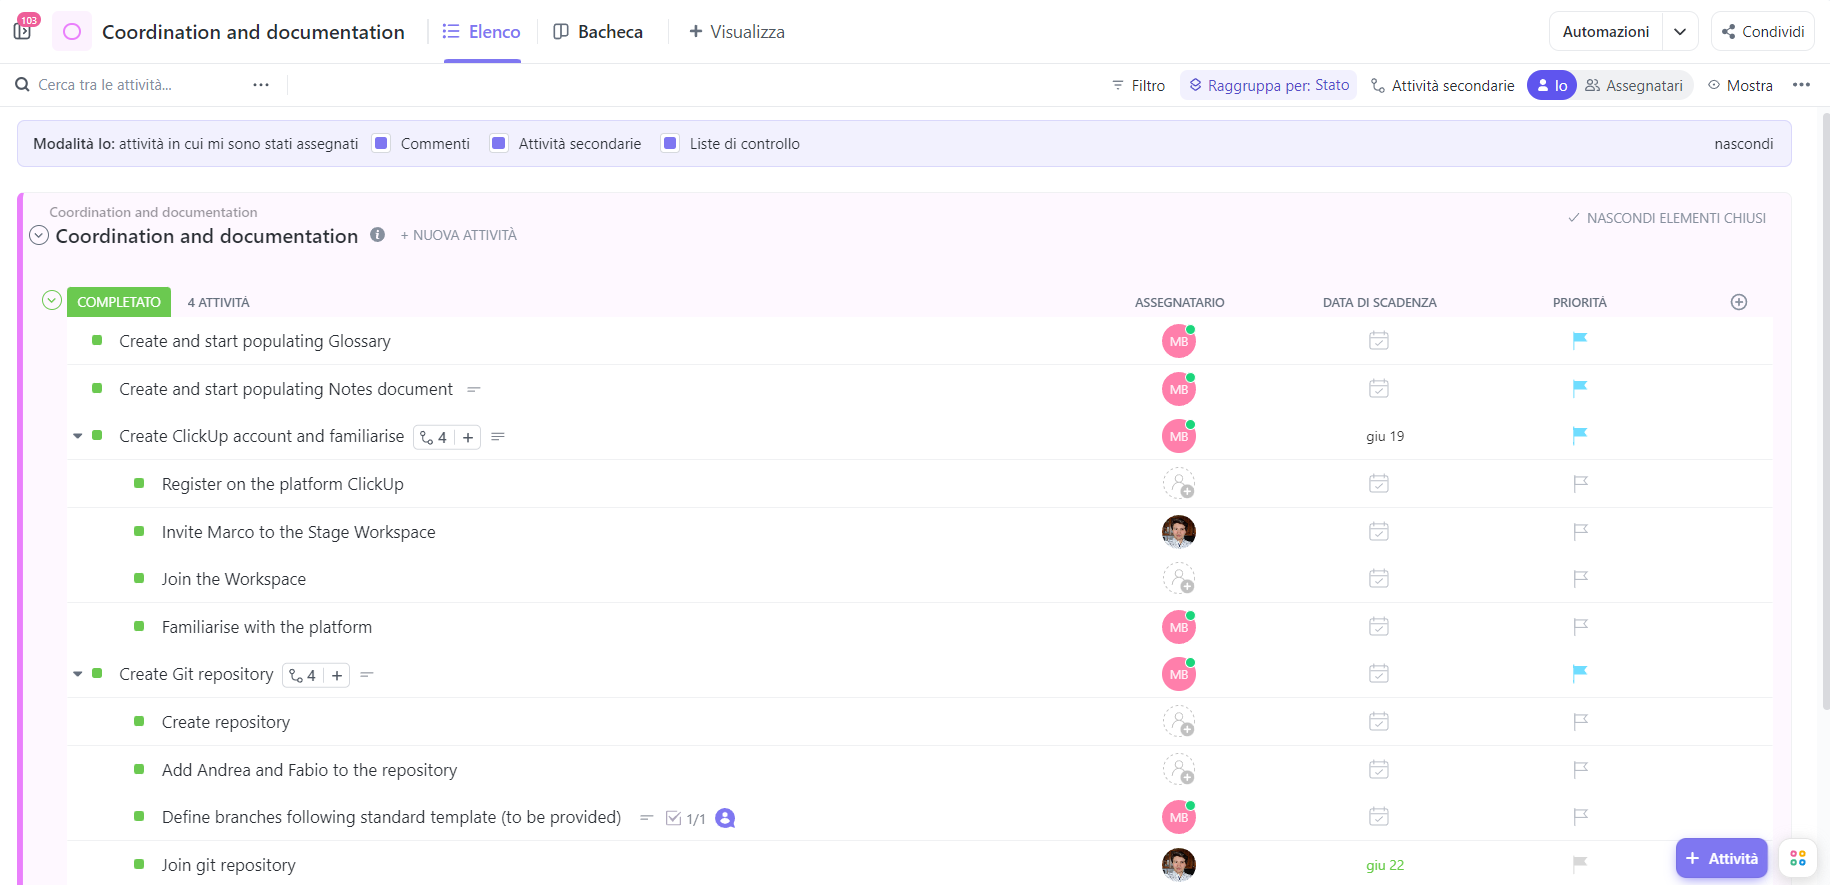
\includegraphics[width=1\textwidth]{images/percorso/coordinamento.png}
    \caption{Board di ClickUp per il processo di coordinamento e documentazione}
    \label{cap:Documentazione}
\end{figure}
\subsection{Daily stand-up meeting}
Durante tutto il percorso di stage, in collaborazione con il tutor aziendale, è stato definito in concomitanza con l'inizio del processo di formazione
è stato definito un processo di \textbf{supporto} in stile \gls{Scrum}{}, andando fissare degli incontri giornalieri di circa 15 minuti finalizzati a:
\begin{list}{*}
    \item \textbf{Monitorare} lo stato di avanzamento delle attività svolte, da svolgere e in corso di svolgimento;
    \item \item \textbf{Risolvere} eventuali dubbi o problemi sorti durante lo svolgimento delle attività;
    \item \textbf{Definire} eventuali miglioramenti o cambiamenti da apportare alle da svolgere o in corso di svolgimento.
\end{list}
\section{Configurazione}
\subsection{Configurazione di un cluster Kafka con Docker Compose}
Dopo aver terminato le attività di formazione su \textbf{Apache Kafka} e \textbf{Docker Compose} 
ho iniziato la configurazione di un \gls{cluster}{} Kafka con Docker Compose. 
\\Seguendo la buona pratica dell'alta affidabilità, descritta del 
paragrafo \ref{sec:alta_affidabilita}, ho configurato un \gls{cluster}{} \textbf{Kafka} con 3 nodi, 1 nodo \textbf{Zookeeper}.\\
Per la configurazione è stato utilizzato il file \ref{lst:file}, di cui ne viene riportato solo la parte relativa alla configurazione di un nodo \textbf{Kafka} gli altri nodi sono configurati in maniera analoga, andando a modificare
solo la porta di ascolto del nodo \textbf{Kafka}.
\pagebreak
\begin{lstlisting}[caption=\texttt{kafka-cluster-compose.yml}, label=lst:file]{kafka-cluster-compose.yml}
  networks:
    kafka-druid:
      name: kafka-druid
      driver: bridge
      external: true
  
  services:
    zookeeper:
      container_name: zookeeper
      hostname: zookeeper
      image: confluentinc/cp-zookeeper:7.4.0
      networks: 
        - kafka-druid
      ports:
        - "2181:2181"
      environment:
        - ZOOKEEPER_SERVER_ID=1
        - ZOOKEEPER_CLIENT_PORT=2181
    kafka:
      image: confluentinc/cp-kafka:7.4.0
      hostname: kafka
      container_name: kafka
      networks:
        - kafka-druid
      ports:
        - "29092:29092"
      environment:
        KAFKA_ADVERTISED_LISTENERS: INTERNAL://kafka:9092,EXTERNAL://localhost:29092
        KAFKA_LISTENER_SECURITY_PROTOCOL_MAP: INTERNAL:PLAINTEXT,EXTERNAL:PLAINTEXT
        KAFKA_INTER_BROKER_LISTENER_NAME: INTERNAL
        KAFKA_ZOOKEEPER_CONNECT: "zookeeper:2181"
        KAFKA_BROKER_ID: 1
        KAFKA_LOG4J_LOGGERS: "kafka.controller=INFO,kafka.producer.async.DefaultEventHandler=INFO,state.change.logger=INFO"
        KAFKA_OFFSETS_TOPIC_REPLICATION_FACTOR: 1
        KAFKA_TRANSACTION_STATE_LOG_REPLICATION_FACTOR: 1
        KAFKA_TRANSACTION_STATE_LOG_MIN_ISR: 1
        KAFKA_AUTHORIZER_CLASS_NAME: kafka.security.authorizer.AclAuthorizer
        KAFKA_ALLOW_EVERYONE_IF_NO_ACL_FOUND: "true"  
\end{lstlisting}   
Da notare all'interno della seguente configurazione l'utilizzo delle immagini\\ \textbf{confluentinc/cp-zookeeper:7.4.0} e \textbf{confluentinc/cp-kafka:7.4.0} invece 
delle immagini ufficiali di \textbf{Apache Kafka} e \textbf{Apache Zookeeper}. \\
Tale scelta è stata fatta \textbf{Confluent Kafka} è oramai diventa una distribuzione molto alla avanguardia e molto utilizzata 
a livello aziendale, anche in Sync Lab. \\
Nonostante ciò tengo a precisare che per i test che verranno elencati di seguito
sono utilizzabili anche le immagini ufficiali di \textbf{Apache Kafka} e \textbf{Apache Zookeeper}.\\
\\
Per la creazione e configurazione del \gls{cluster}{} Kafka con \textbf{Docker Compose} è stato utilizzato il seguente comando:
\begin{lstlisting}[language=bash]
    docker compose -f kafka-cluster-compose.yml up -d
\end{lstlisting}
\subsection{Configurazione del file di enviroment per Apache Druid}
Dopo aver configurato il \gls{cluster}{} \textbf{Kafka}, considerando che \textbf{Apache Druid} è un software che necessita di grandi quantità di risorse per funzionare correttamente, è 
stato necessario configurare il file di enviroment per \textbf{Apache Druid} in modo tale da poter utilizzare il \gls{cluster}{} di \textbf{Apache Druid} in un ambiente che fa uso di \gls{container}{}, minimizzando le risorse a sua disposizione.\\
Per la configurazione è stato utilizzato il seguente file di enviroment ed è stato posto sulla stessa $directory$ del file \textbf{druid-cluster-compose.yml}:
\begin{lstlisting}
# Java tuning
#DRUID_XMX=1g
#DRUID_XMS=1g
#DRUID_MAXNEWSIZE=250m
#DRUID_NEWSIZE=250m
DRUID_MAXDIRECTMEMORYSIZE=3072m
DRUID_SINGLE_NODE_CONF=nano-quickstart

druid_emitter_logging_logLevel=debug

druid_extensions_loadList=["druid-histogram", "druid-datasketches", "druid-lookups-cached-global", "postgresql-metadata-storage", "druid-multi-stage-query", "druid-kafka-indexing-service"]

druid_zk_service_host=zookeeper
druid_lookup_enableLookupSyncOnStartup=true
druid_lookup_lookupTierIsDatasource=false
druid_lookup_lookupTier=_default_tier

druid_broker_cache_useCache=true
druid_broker_cache_populateCache=true
druid_broker_cache_useResultLevelCache=true
druid_broker_cache_populateResultLevelCache=true
druid_cache_useCache=true
druid_cache_populateCache=true
druid_cache_useResultLevelCache=true
druid_cache_populateResultLevelCache=true
druid_metadata_storage_host=
druid_metadata_storage_type=postgresql
druid_metadata_storage_connector_connectURI=jdbc:postgresql://postgres:5432/druid
druid_metadata_storage_connector_user=druid
druid_metadata_storage_connector_password=FoolishPassword

druid_coordinator_balancer_strategy=cachingCost

druid_indexer_runner_javaOptsArray=["-server", "-Xmx1g", "-Xms1g", "-XX:MaxDirectMemorySize=3g", "-Duser.timezone=UTC", "-Dfile.encoding=UTF-8", "-Djava.util.logging.manager=org.apache.logging.log4j.jul.LogManager"]
druid_indexer_fork_property_druid_processing_buffer_sizeBytes=256MiB

druid_storage_type=local
druid_storage_storageDirectory=/opt/shared/segments
druid_indexer_logs_type=file
druid_indexer_logs_directory=/opt/shared/indexing-logs

druid_processing_numThreads=1
druid_processing_numMergeBuffers=1

DRUID_LOG4J=<?xml version="1.0" encoding="UTF-8" ?><Configuration status="WARN"><Appenders><Console name="Console" target="SYSTEM_OUT"><PatternLayout pattern="%d{ISO8601} %p [%t] %c - %m%n"/></Console></Appenders><Loggers><Root level="info"><AppenderRef ref="Console"/></Root><Logger name="org.apache.druid.jetty.RequestLog" additivity="false" level="DEBUG"><AppenderRef ref="Console"/></Logger></Loggers></Configuration>

\end{lstlisting}
È necessario sottolineare che all'interno del file di enviroment, trattandosi di un ambiente che fa uso di \gls{container}{}, 
è stata utilizzata una versione semplificata e minimale di \textbf{Apache Druid} denominata \textbf{nano-quickstart}.\\
\subsection{Configurazione di un cluster Druid con Docker Compose}

\section{Codifica}

\section{Esecuzione e testing}
\newpage
\pagestyle{empty}
\null % o \mbox{} o \phantom{X}
\newpage